\section{Implementation}
This section details the process taken to develop the various discrete components. The final implementation has been developed and tested in a controlled environment using a dedicated wireless network in order to meet the the required ethical standards.

\subsection{Honeypot Application}
\subsubsection{Station Association Sequence}
Using the Lorcon library it is fairly trivial to capture packets and decode them to determine what type they are once inside the Lorcon loop. The packet capture loop takes a callback which is passed a packet structure. To single out the frame type it is a case of indexing in the right location:

\begin{verbatim}
uint8_t packetType = packet->packet_header[HP_80211_TYPE];
\end{verbatim}
The lorcon library also offers a struct with extra info on 802.11 packets, which means the subtype could also be accessed as so:
\begin{verbatim}
struct lorcon_dot11_extra *extra;
extra = (struct lorcon_dot11_extra *)packet->extra_info;
\end{verbatim}
And then accessing the subtype field.

Once we have this information we can use a state style switch statement to determine where in the process of the association sequence we are, and react accordingly to incoming packets.

Firstly the application needs to listen for probe request packets in order to get the SSIDs that nearby devices are searching for. This application is limited in that it only reacts to SSIDs in probe requests that match the SSID passed in as a command line argument. The filter is implemented in the\begin{verbatim} parse_probe_request() \end{verbatim}function and simply compares the SSID in the probe request to the SSID given, where \begin{verbatim}ap_info\end{verbatim} is a struct holding information about the virtual access point:
\begin{verbatim}
if(strcmp(ap_info.ssid, ssid) == 0) {
       ap_info.valid_probe = 1;
return 1;
}
\end{verbatim}
At this point, if a valid probe request has been found, the application pre-checks the authentication type of the AP that the device is probing for by sending a probe response and then parses the authentication response checking whether the Authentication Algorithm is set to Open (i.e. 0). This check is performed so that a virtual access point is not created for devices that are probing for encrypted networks, as the application only handles unencrypted networks currently.

When an open network has been discovered, the application forks and creates a virtual access point using airbase-ng and sends another probe response on behalf of the VAP to speed up the process of associating. It is at this point that the application switches to monitoring traffic, as to meet the ethical guidelines set out by the department, only one device is unwittingly caught in the honeypot as I can ensure it is my device.

\subsubsection{Monitoring Data Packets}

\subsection{Leaky Game}
This application has been developed for Android and mimics the recently popular Flappy Bird style because of its simple nature, and possibility for exploiting the viral hype still surrounding it. It has been developed using Android Java and libgdx to handle the game functions and named Leaky Bird to reflect its actual purpose.

It was developed using the Eclipse IDE due to the support project creation support offered by libgdx tools, the process of which is detailed in a further section. The game was tested in a desktop environment to start with, before being deployed on a Nexus 7 for testing Android specific functionality.
\clearpage
\subsubsection{Project Structure}
Using the libgdx project setup tool removes the need for manually creating the projects and writing the boilerplate code required for the creation of cross-platform games. 

\begin{figure}[h!]
\centering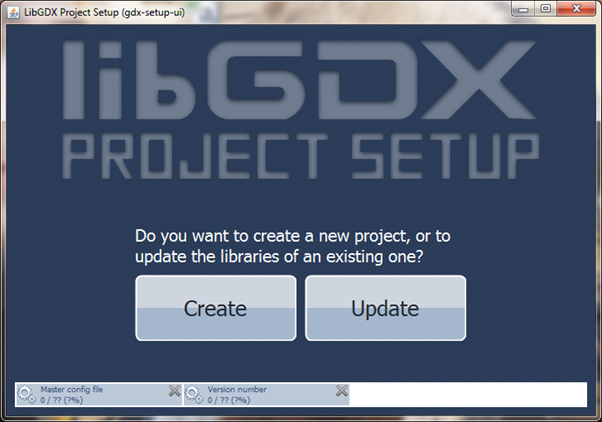
\includegraphics[width=\linewidth]{implementation/figures/gdx-setup-1.png}
\caption{libgdx setup tool.}
\end{figure}

It creates multiple Eclipse projects that link to one main project that holds the game code, thus effectively decoupling any platform specific code from the implementation. The projects created allow you to deploy on Android, desktop, web and iOS using robovm.
\clearpage
\begin{figure}[h!]
\centering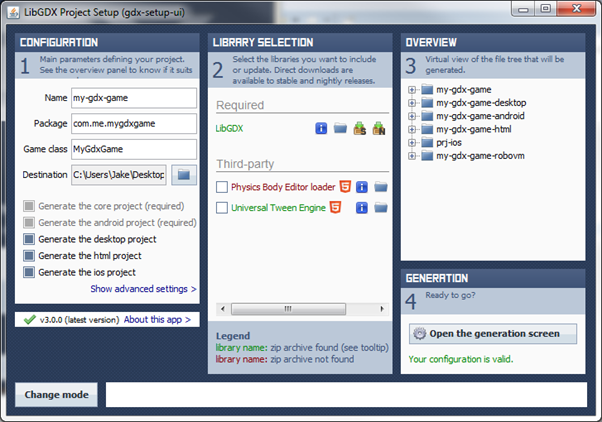
\includegraphics[width=\linewidth]{implementation/figures/gdx-setup-2.png}
\caption{Configuration screen.}
\end{figure}

Which when imported to Eclipse sets the workspace up automatically.

\begin{figure}[h!]
\centering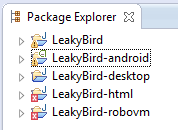
\includegraphics{implementation/figures/gdx-setup-3.png}
\caption{Eclipse project structure.}
\end{figure}
\clearpage
Whilst developing the game it was tested under the desktop deployment, and then when Android specific functions were required it was moved to testing on an actual device.

\subsubsection{Creating Interfaces}
As the Android application utilizes libgdx as it’s graphics library, we need to create a number of interfaces to allow it to use Android specific functions, for example GPS. The process in doing so is relatively straight forward. Firstly you need to create an interface to encapsulate the desired functions and then implement this interface in a class on the Android  side, and pass it through to the constructor of the game. 

In this project the interface takes the naming standard of XResolver, where X is the service it is handling, and the implementation takes the standard of PlatformX where Platform is the deployment platform, e.g. Android, desktop, etc., and X is the service.

If, for example, we were writing a resolver for adding two numbers, we would have an interface in the libgdx project as such:
\begin{verbatim}
public interface AdditionResolver {
    public int add(int a, int b);
}
\end{verbatim}
Then in the Android project implement the interface in a class:
\begin{verbatim}
public class AndroidAddition implements AdditionResolver {
    public AndroidAddition() {
    }

    @Override
    public int add(int a, int b) {
        return a + b;
    }
}
\end{verbatim}
And finally pass it through in the game initialiser in the Android MainActivity:
\begin{verbatim}
initialize(new LeakyBirdGame(androidAddition), cfg);
\end{verbatim}
Remembering to update the constructor of the Game class, then it is ready for use within the application while the game is running. In reality you wouldn’t need something as simple as an addition resolver, this is just to illustrate the steps to take.

\subsubsection{Getting the GPS Co-ordinates}
The application has been developed to report the players location whilst they are playing the game. This required an interface to be written between Android Java and libgdx so that we could take advantage of Android’s GPS support, as noted in the section prior to this about creating interfaces.

The two functions we need the libgdx side of the application to be able to access are the LocationManager class’s getLatitude and getLongitude. The interface to pass to the LeakyBirdGame initialiser is simply:
\begin{verbatim}
public interface GpsResolver {
    public double getGPSLatitude();
    public double getGPSLongitude();
}
\end{verbatim}
It is named resolver due to libgdx being able to create desktop, HTML5 and iOS games from the same source code but with different entry points. Some of these entry points may not have GPS enable so we have to be sure to wrap any calls to this class in a null check. On the Android side we can create a class, AndroidLocationProvider,  that implements this interface and allow the functions to wrap around the two LocationManager calls we need to make in order to get the coordinates. In the constructor of the class we need to get the name of the provider that our game will be using to get the location data, this can either be via GPS or network, the former being finer grained than the latter.
\begin{verbatim}
Criteria criteria = new Criteria();
provider = locationManager.getBestProvider(criteria, false);
\end{verbatim}
Where provider is a class level defined string and criteria is left intentionally default so the application will attempt to get the best provider available.

The two overridden interface functions require nearly identical implementations, with just the longitude/latitude selection switching between them:
\begin{verbatim}
 Location location = locationManager.getLastKnownLocation(provider);
 return location.getLatitude();
\end{verbatim}
As locationManager is passed through to the constructor from the Android MainActivity, it allows us to use a reference to it’s context internally to get the location data during the game’s execution.

In the libgdx project we can now access the GPS, assuming it has been passed through the constructor and named gpsResolver, through the two functions as so:
\begin{verbatim}
game.resolver.showToast(gpsResolver.getGPSLatitude());
\end{verbatim}
This is displayed using an Android Toast resolver that has been implemented in the same manner.


\clearpage